\section{Introduction}
\label{sec:intro}

Large transport vehicles often need to traverse cluttered environments in
which direct passage is blocked by movable obstacles such as pallets, boxes,
or equipment. In these settings, planning must go beyond collision-free
routing. The environment itself must be reconfigured to create a corridor with
sufficient clearance~\cite{liu2023path,stilman2005navigation}. This challenge
arises in warehouse automation, disaster response, and other dense workspaces
where obstacle interaction is unavoidable. The resulting problem is therefore
not only to detect whether passage is blocked, but also to decide how the
blockage can be removed through physical interaction.

As shown in Fig.~\ref{fig:snapshots}, the difficulty becomes sharper when
corridor construction is delegated to a team of smaller mobile robots acting on
behalf of a larger transport platform~\cite{tang2024collaborative,ren2025search}.
The large vehicle defines the required clearance but does not participate in
pushing, so the robot team must identify and execute coordinated contacts that
open a traversable corridor for downstream passage. Cooperative pushing is
therefore a natural mechanism for path clearing, but it also makes feasibility
strongly contact-dependent. Pushing one obstacle can induce coupled motion of
nearby objects, and whether a candidate action succeeds depends on local
geometry, robot size, and obstacle arrangement~\cite{ni2023progressive,liu2025physics}.
As a result, a geometrically plausible clearing sequence may still fail if the
required contacts and motions are not executable.

\begin{figure}[t!]
  \centering
  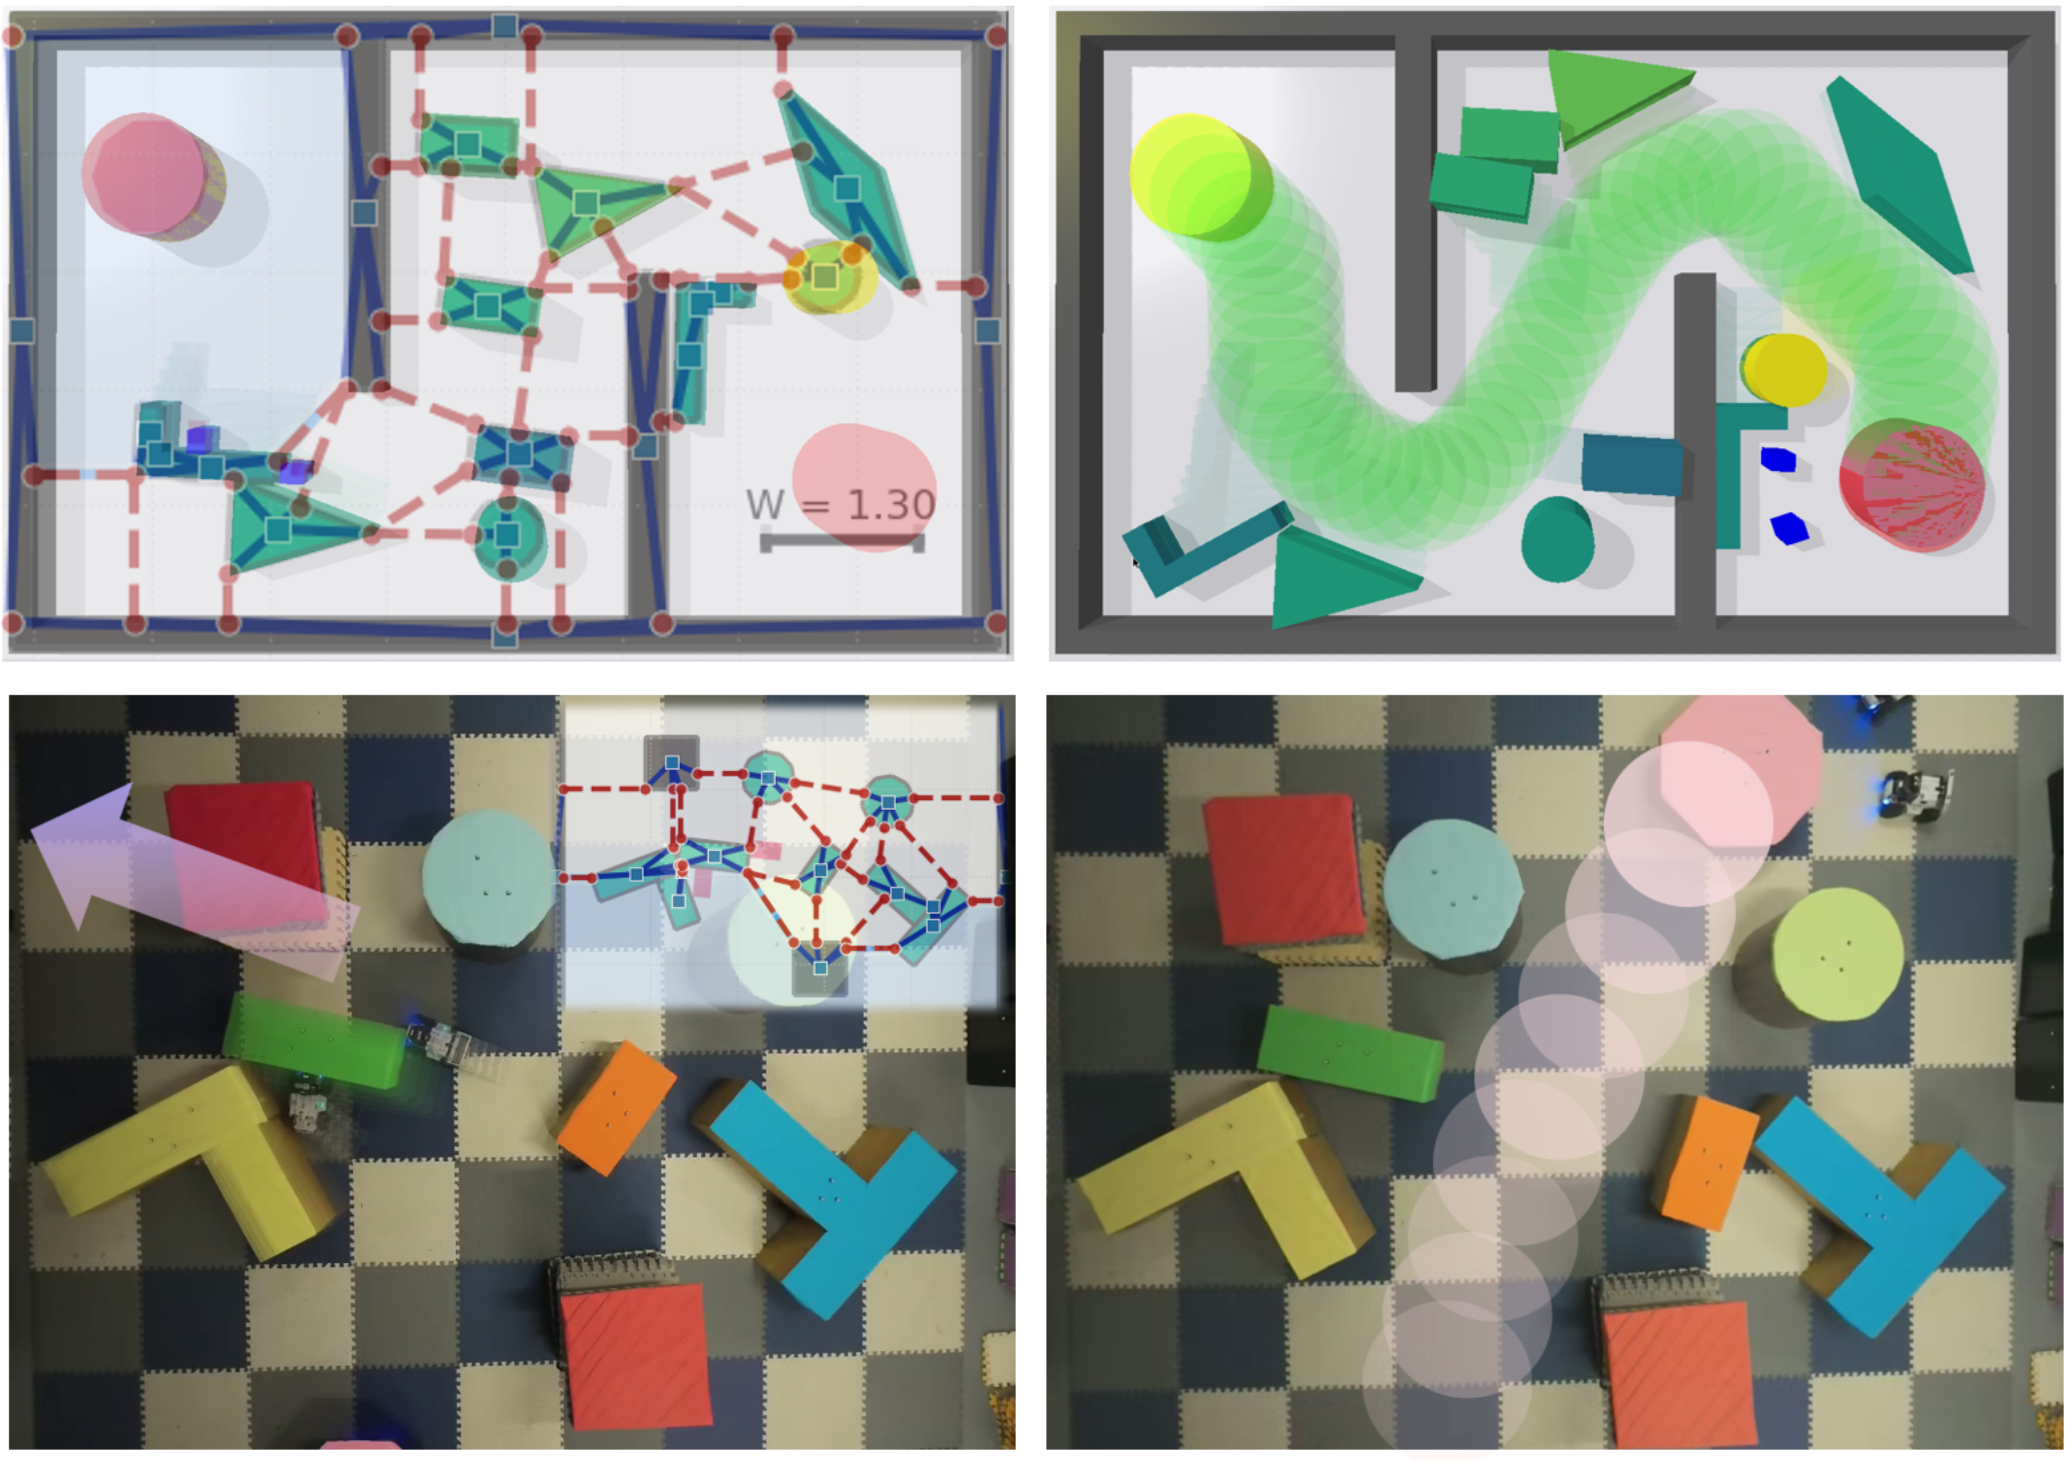
\includegraphics[width=0.9\linewidth]{figures/cover.png}
  \vspace{-0.1in}
  \caption{
    Path clearing in simulation and hardware.
    The robot team selectively opens reachable bottlenecks until a
    $W$-clear corridor emerges.
  }
  \label{fig:snapshots}
\end{figure}

Existing methods typically capture only part of this problem. NAMO-style
approaches reason about obstacle rearrangement and corridor creation, but often
abstract away the contact mechanics that determine whether an intervention can
actually be executed in tightly cluttered scenes~\cite{stilman2005navigation,
yao2024local}. In contrast, collaborative pushing and multi-robot
manipulation methods focus on coordinated contact and force generation, but
usually consider single-object transport or more structured settings~\cite{ni2024physics,
feng2025learning}. Physics-informed planning adds simulation-based validation,
yet this validation is often only loosely coupled to the upstream decision of
which blockage should be addressed first~\cite{lin2019efficient,rouxel2024multi}.
For cluttered path clearing, the missing link is therefore a search procedure
that connects scene-level bottleneck selection to executable multi-robot
contact planning.

This paper addresses that disconnect through a physics-informed corridor hybrid
search, abbreviated PICHS. The WCCG provides a width-aware representation of
whether corridor connectivity already exists, frontier gaps delimit the
reachable intervention set, and short-horizon physical simulation decides which
candidate interventions are executable. PICHS therefore couples bottleneck
selection, candidate generation, and physical validation within one search loop
for collaborative corridor construction.

\begin{figure*}[t!]
  \centering
  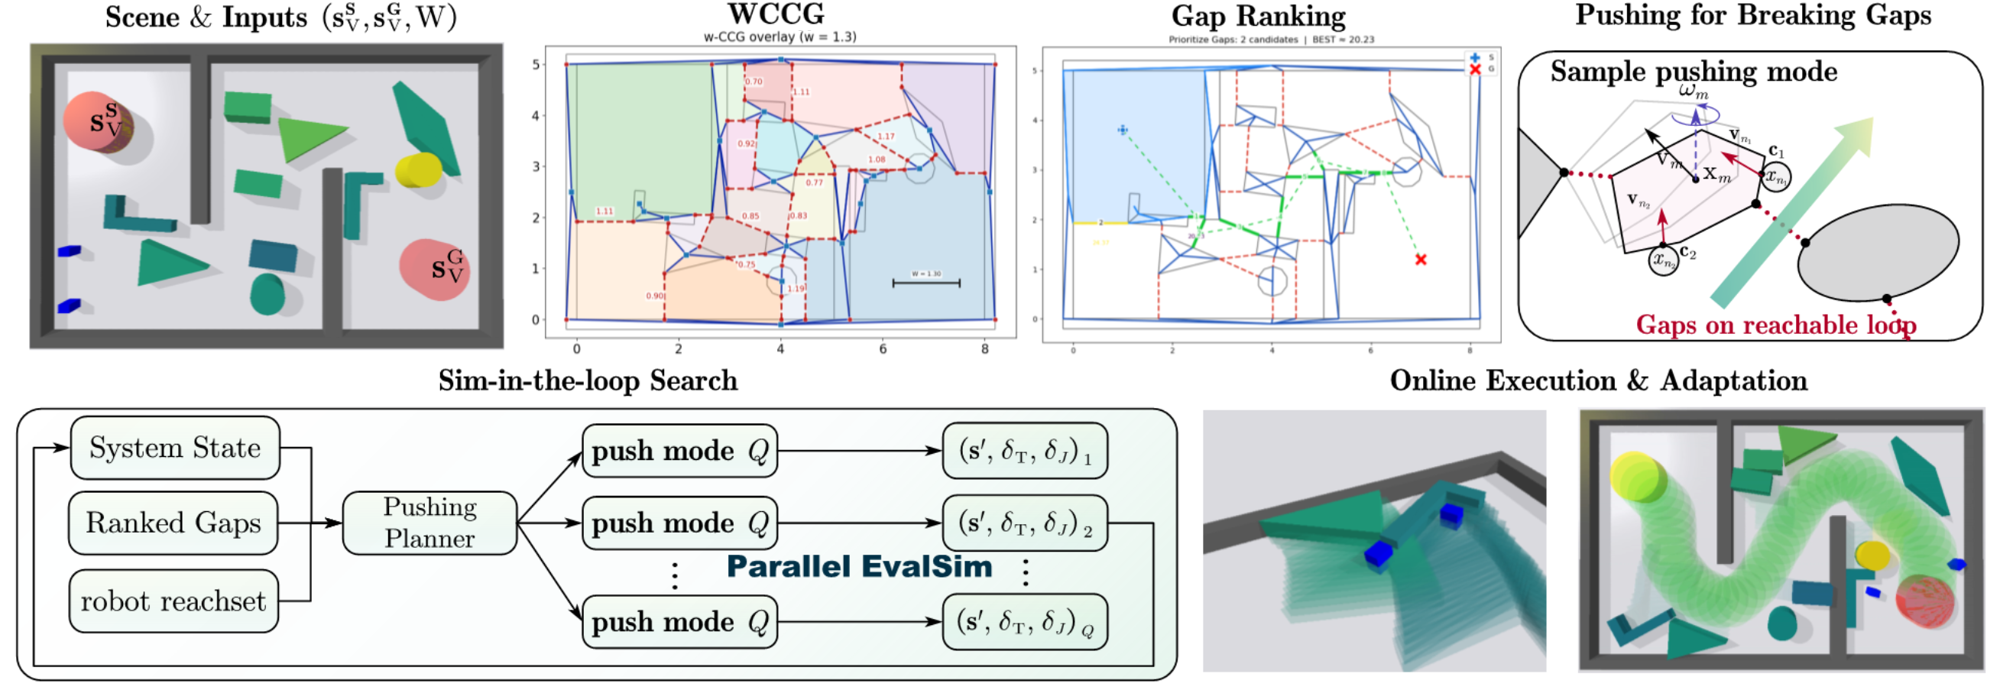
\includegraphics[width=0.95\linewidth]{figures/overall_workshop.png}
  \vspace{-0.1in}
  \caption{Overview of PICHS.
  \textbf{Top:} The WCCG identifies reachable bottlenecks and induces
  gap-conditioned pushing candidates.
  \textbf{Bottom-left:} selective expansion in PICHS.
  \textbf{Bottom-right:} online execution.}
  \label{fig:overall}
  \vspace{-0.2in}
\end{figure*}
